\clearpage
\section{Background}\label{sec-background}

Build systems automate the execution of simple repeatable tasks for individual
users, as well as for large organisations. There are software build systems,
such as \Make~\cite{feldman1979make}, \Shake~\cite{mitchell2012shake} and
\Bazel~\cite{bazel}, as well as various incremental calculation engines, such
as \Excel~\cite{advanced_excel}. In this section we use these four examples to
introduce main domain-specific notions and requirements. Other notable examples
of build systems and their relation to these four will be discussed
in~\S\ref{sec-related} and~\S\ref{sec-conclusions}.

\subsection{The venerable \Make}

\Make\footnote{There are numerous implementations of \Make and none comes with a
formal specification. In this paper we therefore use a simple and sensible
approximation to a real \Make that you might find on your machine.} was developed
more than 40 years ago to automatically build software libraries and executable
programs from source code. It uses \emph{makefiles} to describe build tasks,
typically referred to as \emph{build rules}, and their dependencies in a simple
text form. For example:

\begin{minted}[frame=single]{makefile}
util.o: util.h util.c
    gcc -c util.c

main.o: util.h main.c
    gcc -c main.c

main.exe: util.o main.o
    gcc util.o main.o -o main.exe
\end{minted}

\noindent
The above makefile lists three tasks: (i) compile a utility library comprising
files \cmd{util.h} and \cmd{util.c} into \cmd{main.o} by
executing\footnote{In this example we treat \cmd{gcc} as a pure function for the
sake of simplicity. In reality there are multiple versions of \cmd{gcc} and the
actual binary that is used to compile and link files is also listed as a task
dependency.} the command \cmd{gcc -c util.c}, (ii) compile the main source file
\cmd{main.c} into \cmd{main.o}, and (iii) link object files \cmd{util.o} and
\cmd{main.o} into the executable \cmd{main.exe}. The makefile contains the
complete information about the task \emph{dependency graph}, which is shown in
Fig.~\ref{fig-make}(a).

\begin{figure}[h]
\begin{subfigure}[b]{0.32\linewidth}
\centerline{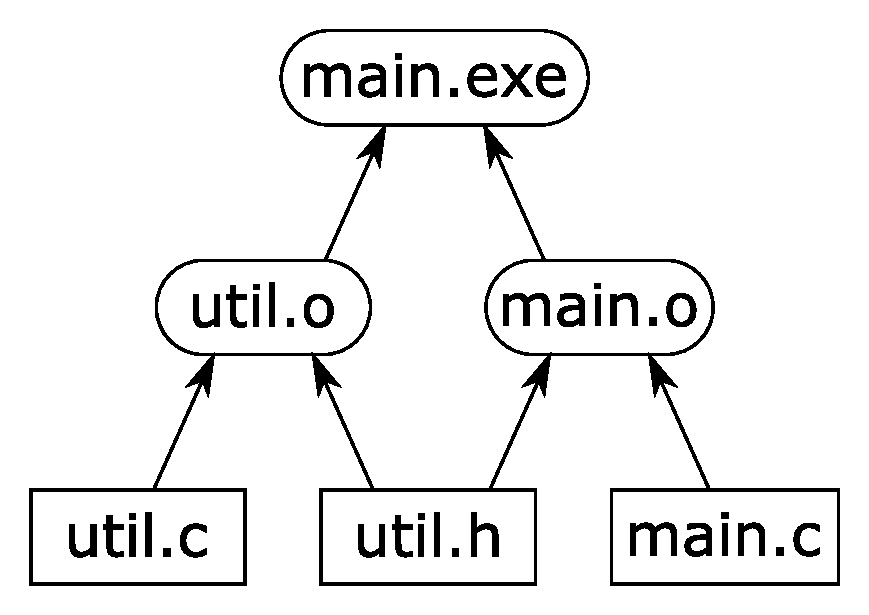
\includegraphics[scale=0.28]{fig/make-example.pdf}}
\caption{A dependency graph}
\end{subfigure}
\begin{subfigure}[b]{0.32\linewidth}
\centerline{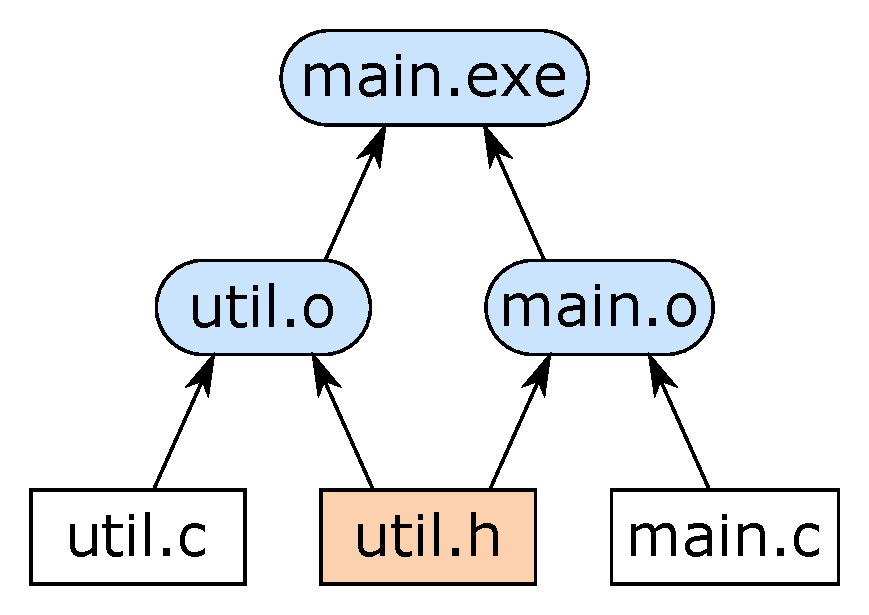
\includegraphics[scale=0.28]{fig/make-example-full.pdf}}
\caption{A full rebuild}
\end{subfigure}
\begin{subfigure}[b]{0.32\linewidth}
\centerline{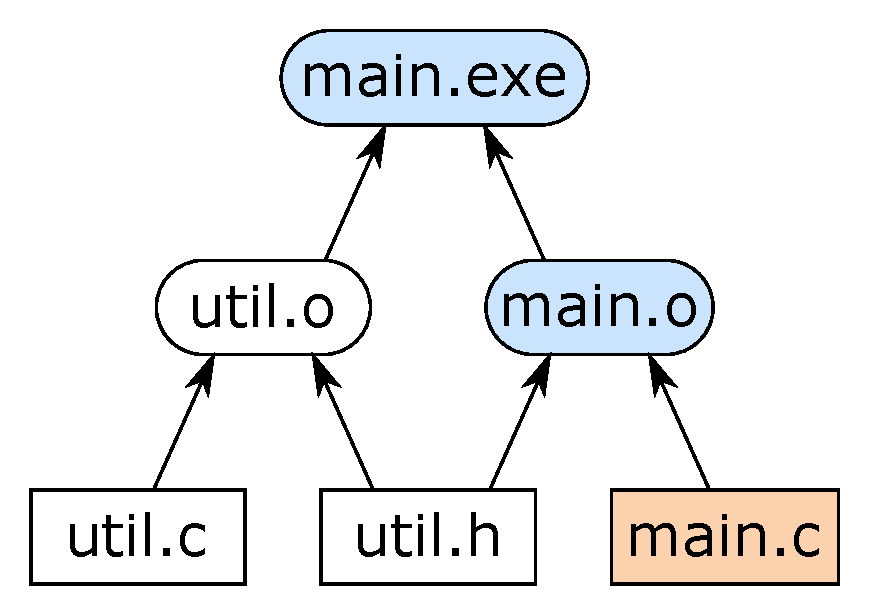
\includegraphics[scale=0.28]{fig/make-example-partial.pdf}}
\caption{A partial rebuild}
\end{subfigure}
\caption{A dependency graph and two build scenarios. Input files are shown as
rectangles, intermediate and output files are shown as rounded rectangles. Dirty
inputs and files that are rebuilt are highlighted.
\label{fig-make}}
\end{figure}

If the user modifies the sources of the utility library and runs \Make, it will
perform a full rebuild, because all three tasks transitively depend on the
library, as illustrated in Fig.~\ref{fig-make}(b). On the other hand, if the
user modifies \cmd{main.c} then a partial rebuild is sufficient: indeed, the
file \cmd{util.o} does not need to be rebuilt, since its inputs have not
changed, see Fig.~\ref{fig-make}(c). Files that have changed since the previous
build are called \emph{dirty}.

The requirement to execute tasks \emph{at most once} and only if they
\emph{transitively depend on dirty inputs} is essential for build systems,
their raison d'\^etre. We will call build systems that satisfy this requirement
\emph{minimal}.

To achieve minimality \Make relies on two key ideas. First, it uses \emph{file
modification time} to detect the files that are dirty: a file is marked dirty if
it was modified after the previous build. Second, it constructs a complete task
dependency graph from the information contained in the makefile and executes
tasks in the \emph{topological order}.

...

\subsection{\Excel: a build system in disguise}

...

\Shake

\begin{figure}[h]
\centerline{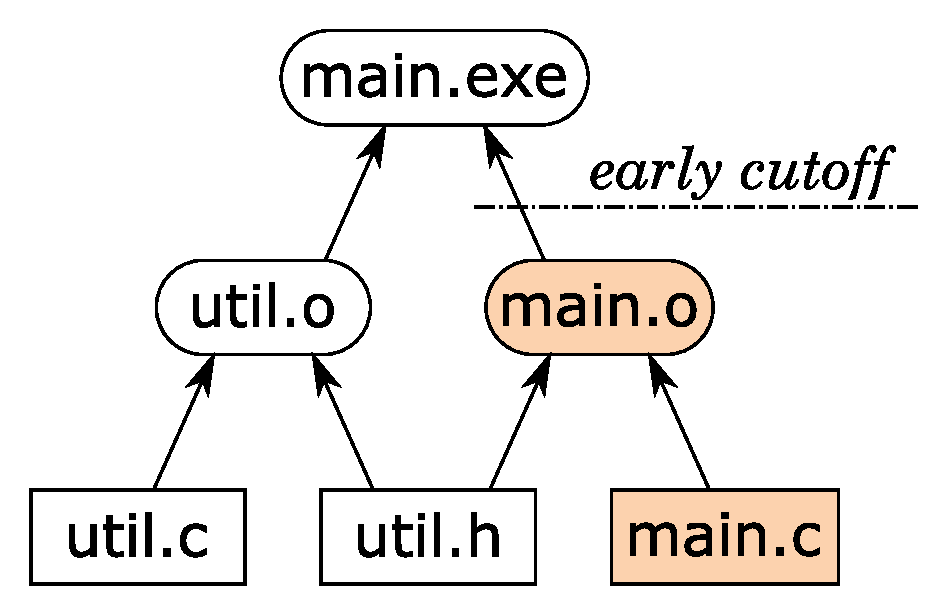
\includegraphics[scale=0.28]{fig/make-example-cutoff.pdf}}
\caption{An early cut-off example.\label{fig-cutoff}}
\end{figure}



...

\Bazel

...

\begin{itemize}
    \item Many build systems, such as the venerable \Make, need to know the
    complete \emph{dependency graph} between tasks at the start of the build
    process. This makes it possible to analyse the graph ahead of time, which
    helps with efficient task scheduling but is fundamentally limited: parts of
    the dependency graph can often be discovered only during the build process,
    i.e. the dependency graph is \emph{dynamic}, not \emph{static}.

    \item When build systems are used by large teams, different team members
    often end up executing exactly the same tasks on their local machines.
    A \emph{cloud build system} can speed up builds dramatically by
    transparently sharing build results among team members. Furthermore, cloud
    build systems allow one to perform \emph{shallow builds} that materialise
    only end build products on a local machine, leaving all intermediates in the
    cloud. This is a significant optimisation compared to \emph{deep builds}
    that require all transitive dependencies of an end build product to be
    locally available. Non-cloud build systems cannot support shallow builds.

    \item Some build systems, e.g. \Buck, require all tasks to be
    \emph{deterministic}, i.e. produce exactly the same output when run on the
    same inputs. However, not all tasks are deterministic, and there are build
    systems that support \emph{non-determinism}. A simple example is \Excel's
    \textsf{RANDBETWEEN(low, high)} that returns a random integer in the
    interval \textsf{[low, high]}.

    \item If a build system executes a task and the result is unchanged from the
    previous build, it is unnecessary to execute the dependent tasks. We call
    this optimisation \emph{early cut-off}. Not all build systems support early
    cut-off: \Make and \Excel do not, whereas \Shake and \Buck do.

    \item Most build systems track changes of inputs and intermediate results,
    executing dependent tasks whenever they change, but some build systems can
    also track changes in the tasks themselves: if a task has changed, the build
    system will execute it. For example, when a cell's formula has changed,
    \Excel will recompute its value and propagate the changes. We call this
    \emph{self-tracking}. Self-tracking is uncommon in software build systems,
    where one often needs to manually initiate a rebuild of all tasks even if
    just a single task has changed.

    \item Most build systems persistently store auxiliary \emph{build
    information} for profiling and optimisation purposes: \Make stores file
    modification times, \Shake stores the discovered dynamic dependency graph,
    \Bazel and other cloud build systems store information about inputs and
    outputs of previously executed tasks, etc.
\end{itemize}

This paper presents a purely functional abstraction for build systems that
allows us to express all the above intricacies of build systems and design
complex build systems from simple primitives. The presented abstraction fits in
just two lines of Haskell code, which are explained
in~\S\ref{sec-abstractions}:

\begin{minted}{haskell}
type Compute c k v = @\std{forall}@ f. c f => (k -> f v) -> k -> Maybe (f v)
type Build c i k v = Compute c k v -> k -> Maybe i -> Map k v -> (i, Map k v)
\end{minted}


Below we define basic notions used in build systems and other similar domains,
for example, spreadsheets.

\subsection{Keys, values, hashes and store}

\emph{Keys} are used to distinguish \emph{values}. In build systems keys are
typically filenames, e.g. \textsf{src/file.c}, whereas values are file contents
(a C program source code in this case). In spreadsheets keys are cell names,
e.g. \textsf{A1}, and values are numbers, text, etc. that are typically displayed
inside cells. We will use type variables \hs{k} and \hs{v} to denote keys and
values, respectively.

A \emph{store} associates keys to values. It is convenient to assume that a store
is total, i.e. it contains a value for every possible key. We therefore also
assume that the type of values is capable of encoding values corresponding to
non-existent keys (missing files or empty cells).

We use a cryptographic \emph{hash function} \hs{hash :: v -> Hash} for
efficient tracking and sharing of build results.

\subsection{Input, intermediate and output values}

Some values must be provided by the user as \emph{input}. For example,
\textsf{src/file.c} can be edited by the user who relies on the build system to
compile it into \textsf{obj/file.o}. Similarly, the user can input \textsf{A1 = 5}
and \textsf{B1 = 9} expecting the spreadsheet to compute their sum in \textsf{C1},
i.e. \textsf{C1 = 14}.

In the above examples, \textsf{obj/file.o} and \textsf{C1} are \emph{output} values.

In some situations we might also need the notion of \emph{intermediate} values,
which are not interesting for the user but are produced in the process of turning
inputs into outputs. For example, the user might only be interested in the
executable \textsf{bin/file.exe} obtained by linking \textsf{obj/file.o} with
standard libraries, in which case \textsf{obj/file.o} can be considered an
intermediate value.

\subsection{Non-deterministic computations}

Build systems and spreadsheets compute output values from input and intermediate
values. In the most typical case, these \emph{computations} are \emph{functions},
such as \textsf{C1 = A1 + B1}, i.e. their result is uniquely determined by the
input values. However, in general they can be \emph{relations}, i.e. have
multiple valid results. A spreadsheet example: \textsf{A2 = A1 + RANDOM(1,6)}.
This computation has six valid results for each input value \textsf{A1}. In
build systems, the object file \textsf{obj/file.o} is sometimes not uniquely
determined by the source \textsf{src/file.c} -- different compiler runs may
produce different valid results.

\subsection{Dynamic dependencies}

...

\todo{AM}{Add two examples: include files and cyclic spreadsheet computations.}

\subsection{Requirements for build systems}

\begin{itemize}
    \item Correctness
    \item Minimality
    \item Support for sharing and skipping intermediate values
\end{itemize}
...
